\documentclass[12pt]{article}
\usepackage[margin=1in]{geometry}
\usepackage{amsmath}
\usepackage{graphicx}
\usepackage{setspace}
\usepackage{subcaption}
\usepackage{listings}
\usepackage[italicdiff]{physics}
\usepackage{natbib}
\usepackage{epstopdf}
\lstset{breaklines=true, tabsize = 3}

\author{Jonathan Bunton}
\title{Time-Dependent Behavior of Heat \\ in a Cubic Satellite}
\date{\today}

\begin{document}
\maketitle
\onehalfspacing
\begin{abstract}
Before launching objects into low orbit space, it is prevalent to study their expected behavior in given conditions.  One such behavior is the expected temperature variations at the time of launch, moving foward in time.  To determine this behavior, we can utilize the fact that in general, the temperature of a material over time $T(x,y,z,t)$ is governed by the heat equation. \cite{heateq} This partial differential equation is given by:
\begin{equation*}
\nabla^2T = \frac{1}{\alpha}\dv{T}{t}
\end{equation*}
To begin to solve this equation, we require proper boundary conditions. In this particular case, we consider a tidally locked 0.1 meter cubic mass of polystyrene foam, coated with polysilicon, initially at 30 K.  Centered in the polystyrene foam is a 0.4 meter cubic aluminum mass which stays at a constant 100 K. This system serves as our ``satellite."  To calculate the change in temperature over time, we consider two relevant methods of heat transfer: conduction and radiation.  All outside faces of the satellite are able to emit radiation, and we assume the face nearest the sun absorbs thermal energy, with both absorption and emission values being governed by the Stefan-Boltzmann law. \cite{sblaw}  The conduction of heat is considered at all points on the satellite, governed by the Laplacian operator in the heat equation.

To numerically calculate these values, we discretize our space by dividing the satellite into a 3D mesh.   To find values for $\nabla^2T$, we utilize a central difference method to approximate the second derivatives at each point.  We consider this and the diffusivity constant, $\alpha$, which gives a material's tendency to conduct heat, alongside the radiation terms on the satellite faces to find a value for $\dv{T}{t}$.

Once this value is determined at a particular time, we need only numerically integrate to find the values at points further in time.  In this project, we use fourth-order Runge-Kutta to perform accurate integration of these values in time.\cite{rk4}  The resulting integration yields the temperature behavior at all points over a set number of timesteps.  The results differ from our expected steady-state behavior outlined in prior work \cite{lastpaper}, but this work neglected the diffusivity and specific heats of each material that govern the satellite components' susceptibility to changes in temperature.  By scaling up these constants from their true values, we can see effects occur much faster and make accurate comments on the temperature trends without wasting computing power.  These trends indicate decaying exponential functions govern the temperature along the faces of the box.  In addition, the interior 100 K aluminum box acts initially as a heat source to the 30 K foam, but as time goes on, the box acts more as a heat sink for the warming foam outside.
\end{abstract}
\section*{Results}
We have oriented the satellite with the axes $i, j,k$ as shown in figure \ref{justbox}.  The face marked with yellow, $i = 1$, is facing the sun.  This orientation is consistent through all plots.

\begin{figure}
\begin{center}
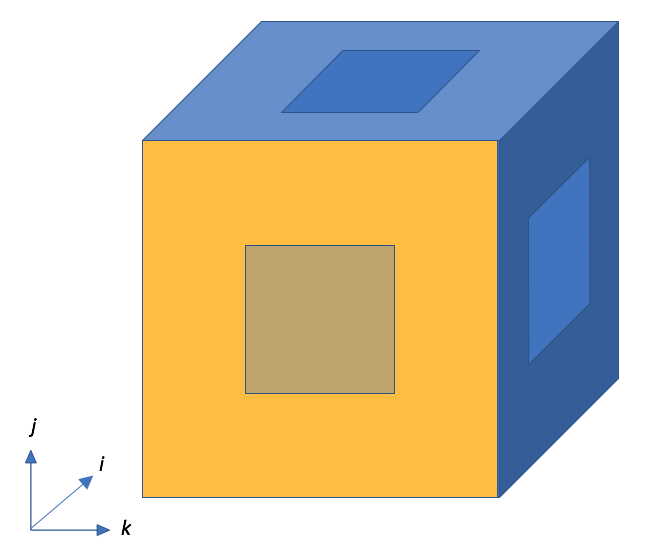
\includegraphics[width = 0.5\textwidth]{../pics/justbox.png}
\end{center}
\caption{\label{justbox} An image indicating the orientation of our cubic satellite in space, alongside the position of the interior cube, marked on the outer faces.}
\end{figure}
\subsection*{Temperature Distribution Results}
Because the results are effectively five-dimensional ($x$, $y$, $z$ in space, with a temperature and time at each point), the results are plotted as planes through the satellite cube at particular times.  All plots are done in this manner, with an image indicating the particular plane cut through the satellite.  For reference, the initial conditions placed on the system are shown in fig. \ref{initial}.

\begin{figure}[h!]
\begin{center}
\begin{subfigure}{0.3\textwidth}
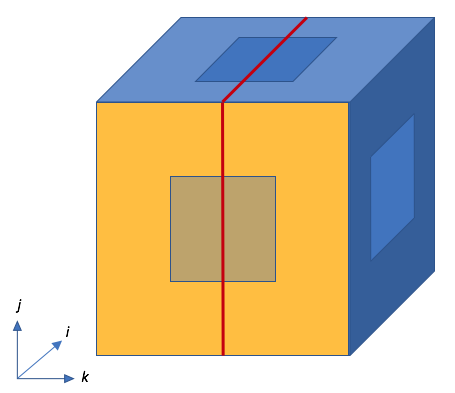
\includegraphics[width=\linewidth]{../pics/centeredkpic.png}
\caption{\label{centeredjpic}}
\end{subfigure}
\begin{subfigure}{0.6\textwidth}
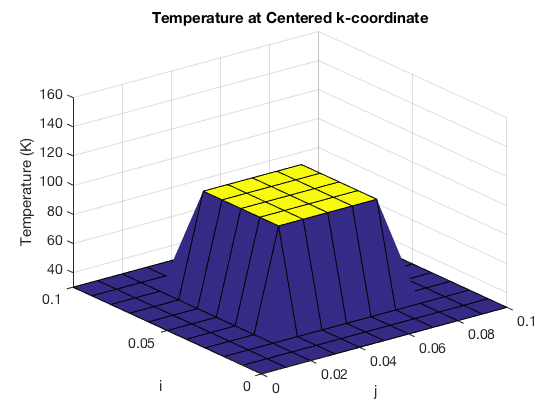
\includegraphics[width=\linewidth]{../pics/initialconditionscenteredk.png}
\caption{\label{centeredj}}
\end{subfigure}
\caption{\label{initial}A plot of the initial temperature distribution through a cross-section at the center of the $k$-axis.}
\end{center}
\end{figure}

Using the constants for the specific heat and diffusivity of the various materials within the satellite, a cut through all $i$, $j$, and $k$ planes are identical and shown after approximately 15 minutes in fig. \ref{15mincenteredk}.  Most noticeable is the lack of heat build up on the face nearest the sun, where one would expect a more prominent effect.  Because polysilicon has a very high specific heat and is very dense, it does not absorb the radiated heat from the sun effectively. \cite{polysilicon}  In addition, polystyrene's incredibly low diffusivity constant indicates the material does not conduct heat very quickly, which is also reflected by the amount of time required to reach the distribution shown. \cite{polystyrene}

\begin{figure}[h!]
\begin{center}
\begin{subfigure}{0.3\textwidth}
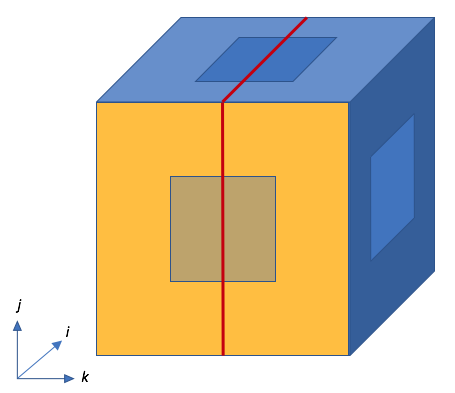
\includegraphics[width=\linewidth]{../pics/centeredkpic.png}
\caption{\label{15minkpic}}
\end{subfigure}
\begin{subfigure}{0.6\textwidth}
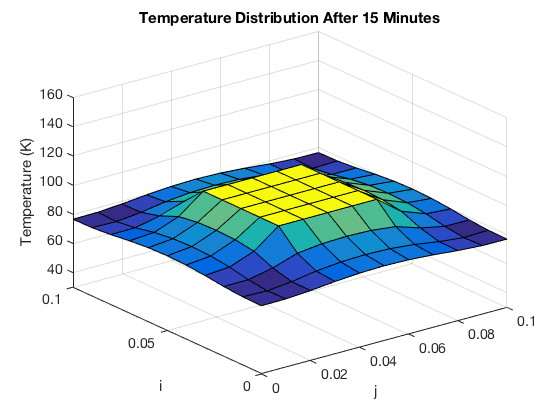
\includegraphics[width=\linewidth]{../pics/15mincenteredk.png}
\caption{\label{15mink}}
\end{subfigure}
\caption{\label{15mincenteredk}A plot of temperature through a cross-section at the center of the $k$-axis.  This distribution is shared across the other two cross-sections, showing an exponential decay away from the 100 K satellite center.  In this case, the center acts as a source of heat, and the heat absorbed from the sun is negligible.}
\end{center}
\end{figure}

Moving further forward in time leads to a nearly flat line temperature distribution at 100 K.  This makes sense in the context, as the only release of heat is via radiation from the polysilicon layers which do so poorly.  The poor radiation keeps the heat generated by the internal box contained in the system as it slowly raises (through the poor diffusivity in the polystyrene) in temperature to almost level with the 100 K, as shown in fig. \ref{30mincenteredk}, which represents the distribution after approximately 30 minutes.

\begin{figure}[h!]
\begin{center}
\begin{subfigure}{0.3\textwidth}
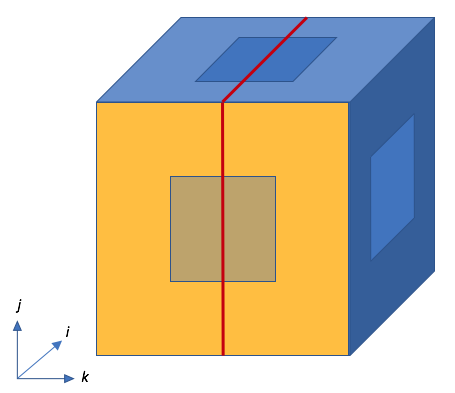
\includegraphics[width=\linewidth]{../pics/centeredkpic.png}
\caption{\label{30minkpic}}
\end{subfigure}
\begin{subfigure}{0.6\textwidth}
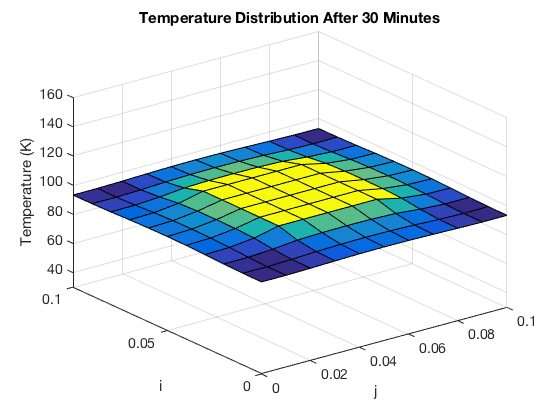
\includegraphics[width=\linewidth]{../pics/30mincenteredk.png}
\caption{\label{30mink}}
\end{subfigure}
\caption{\label{30mincenteredk}A plot of temperature through a cross-section at the center of the $k$-axis.  This distribution is shared across the other two cross-sections, showing a very slight exponential decay from the center, where the faces radiate away heat.}
\end{center}
\end{figure}

Previous work suggested a different shape for eventual temperature distribution, but this work failed to consider the type of material at hand.  If we instead set this simulation's material-based constants (density, diffusivity, specific heat) to 1, it would model a system more closely parallel to the one analyzed in previous work.  The result is shown in fig. \ref{homogenouscenteredk}.

\begin{figure}[h!]
\begin{center}
\begin{subfigure}{0.3\textwidth}
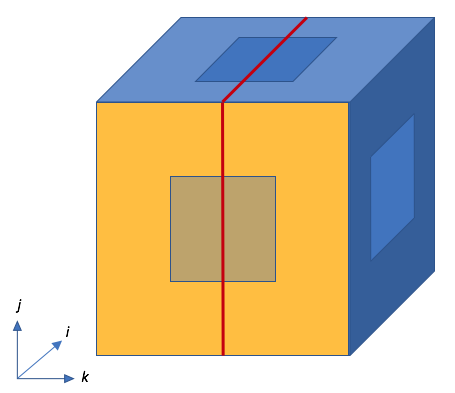
\includegraphics[width=\linewidth]{../pics/centeredkpic.png}
\caption{\label{homokpic}}
\end{subfigure}
\begin{subfigure}{0.6\textwidth}
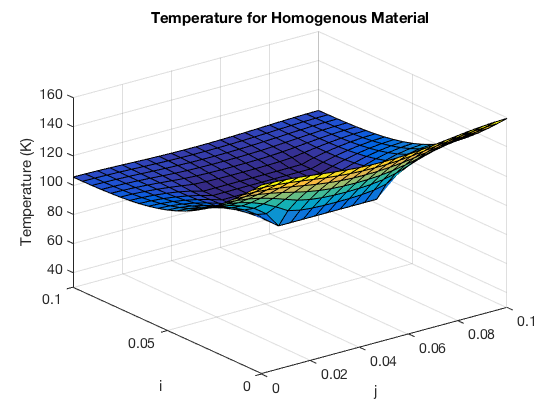
\includegraphics[width=\linewidth]{../pics/homogenous.png}
\caption{\label{homok}}
\end{subfigure}
\caption{\label{homogenouscenteredk}A plot of temperature through a cross-section at the center of the $k$-axis in a homogenous material.  The result is a slight exponential decay moving away from the sun, with the aluminum box acting effectively as a heat sink.}
\end{center}
\end{figure}
\begin{figure}[h!]
\begin{center}
\begin{subfigure}{0.3\textwidth}
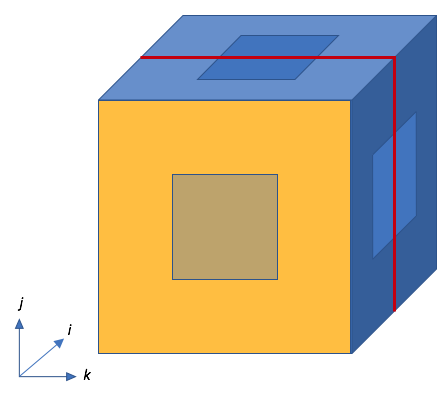
\includegraphics[width=\linewidth]{../pics/centeredipic.png}
\caption{\label{homoipic}}
\end{subfigure}
\begin{subfigure}{0.6\textwidth}
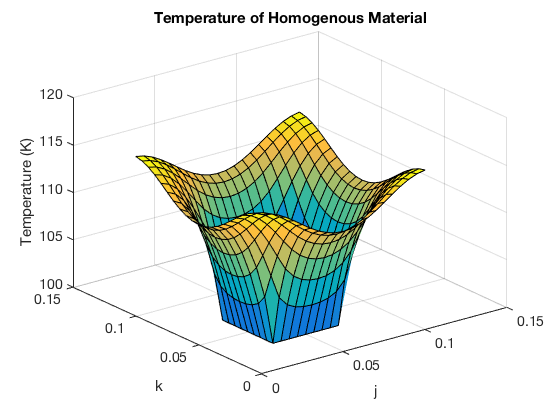
\includegraphics[width=\linewidth]{../pics/homoi.png}
\caption{\label{homoi}}
\end{subfigure}
\caption{\label{homogenouscenteredi}A plot of temperature through a cross-section at the center of the $i$-axis in a homogenous material.  Clear exponential decays show the eventual role of the center aluminum as a heat sink, rather than source.}
\end{center}
\end{figure}

In the $i$-axis cross section shown in fig. \ref{homogenouscenteredi} the pronounced dip in the center of each face is clear.  This effect occurs because center face points are in contact with more points in the satellite than the edges or corners, meaning in the central difference method they are averaged with fewer internal values.  Because in our simulation we considered space a vacuum with nothing to conduct thermal energy from, our central difference method effectively averages with less internal points, causing these points to hold heat more than others.
 
\subsection*{Discussion}
Ultimately, these results point to a very thermally stable satellite if crafted from the materials laid out in our assumptions.  The long term behavior shows that the primary source of heat in the system is the center aluminum box, meaning if it truly does operate as assumed at a constant temperature of 100 K, the remainder of the box will slowly rise to match the 100 K.  100 K is relatively low in temperature, which means the box is safe in low orbit.  

Compared to previous simulations, this result is strikingly different.  This mostly comes into effect as a result of the simplifying assumptions made in previous work, where the type of material in question had no bearing on the long term behavior, which is not entirely true.  As proof of this as the reason for discrepancy, a quick simulation of the same satellite but instead cast as a homogenous material with all characteristic constants set to one yields results closer to previous simulations.

\pagebreak
\bibliographystyle{plain}
\bibliography{sources}
\pagebreak
\section*{Appendix}
Attached is the source code for this project, written in Fortran.
\lstinputlisting[language=Fortran]{../theateq.f90}
\lstinputlisting[language=Fortran]{../derivatemp.f90}
\subsection*{MATLAB Plotting Script}
\lstinputlisting[language=Octave]{../makeplots.m}
\end{document}